\section{Vorbereitungsfragen}
\label{sec:Vorbereitungsfragen}

Teil der Vorbereitung ist es zwei Szenarien der Raumbeleuchtung für ein Musterbüro zu berechnen. 
Szenario 1 entspricht 'Good Practice' Szenario zwei soll den 'Worst Case' abdecken.
Raumabmessungen und Vorgaben sind der Versuchsanleitung zu entnehmen.

\begin{figure}[H]
    \centering
    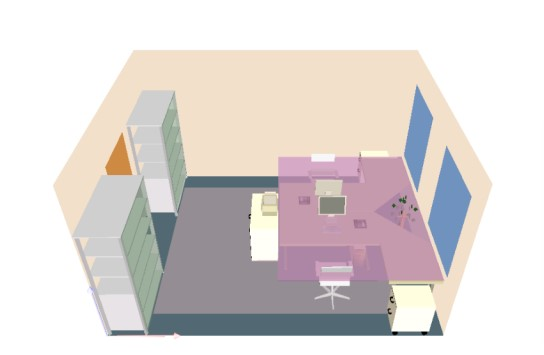
\includegraphics[width=0.7\textwidth]{Abbildungen/Raumaufbau.jpg}
    \caption{Aufbau des Musterbüros [Versuchsanleitung] }
    \label{fig:abb5}
\end{figure}


K1 wird mit \autoref{eq:230624_k1} berechnet, wobei $A'_F$ die lichtdurchlässige Fläche und $A_F$ die Fläche der Rohbauöffnung darstellt.
Die Rahmenfläche lässt sich mittels der Rahmendicke und dem gegebenen Umfang der Fenster berechnen: 

\begin{equation}
    A_{Rahmen} = U_{Fenster} \cdot d_R
\end{equation}

Daraus wiederum lässt sich die lichtdurchlässige Fläche berechnen:  


\begin{equation}
    A'_F = A_{Fenster} - A_{Rahmen}
\end{equation}

Für 'Good Practice' wird von einer Rahmendicke von $d_{R,GP} = 5cm$ und für den 'Worstcase' $d_{R,WC} = 7 cm$ ausgegangen.
Daraus ergeben sich $k_{1,GP} = 0,8542$ und $k_{1,WC} = 0,7958$ welche auch in \autoref{tab:230426_Korrektur-Faktoren} zusammengefasst werden.
K2 kann mittels einer Tabelle in der DIN 5034-3 abgeschätzt werden.
Der Best Case der Verschmutzung wäre $k_2 = 0,9$ der Worst Case hingegen beträgt $k_2 = 0,5$.
Da 'Good Practice' allerdings nicht der best Case ist, wird von $k_{2,GP} = 0,8$ ausgegangen.
Der Korrekturfaktor für nicht senkrechten Lichteinfall hat einen Pauschalwert von $k_3 = 0,85$, der Transmissionsgrad wird als $T = 0,9$ vorgegeben.
Nun kann der effektive Transmissionsgrad mit \autoref{eq:230624_Lichttransmissionsgrad} berechnet werden und wird, so wie alle anderen Faktoren, in \autoref{tab:230426_Korrektur-Faktoren} zusammengefasst.


\begin{equation}
    k_1 = \frac{A'_F}{A_F}
    \label{eq:230624_k1}
\end{equation}

\begin{equation}
    \tau = k_1 \cdot k_2 \cdot k_3 \cdot T
    \label{eq:230624_Lichttransmissionsgrad}
\end{equation}


\begin{table}[H]
    \caption{Zusammenfassung der Korrektur Faktoren}
    \centering
    \begin{tabular}{|c|c|c|}
    \hline
    \rowcolor[HTML]{70AD47} 
    Korrektur Faktor                                & Good Practice & Worst Case \\\hline
    \rowcolor[HTML]{CFE5A8} 
    $k_1$ - Rahmen und Sprossen                     & 85,42\%       & 79,58\%    \\\hline
    \rowcolor[HTML]{A9D08E} 
    $k_2$ - Verschmutzung                           & 80\%          & 50\%       \\\hline
    \rowcolor[HTML]{CFE5A8} 
    $k_3$ - nicht senkrechter Lichteinfall          & 85\%          & 85\%       \\\hline
    \rowcolor[HTML]{A9D08E} 
    T - Transmissionsgrad                           & 90\%          & 90\%       \\\hline
    \rowcolor[HTML]{CFE5A8} 
    $\tau$ - Effektiver Lichttransmissionsgrad      & 52,28\%       & 30,44\%   \\\hline
    \end{tabular}
    \label{tab:230426_Korrektur-Faktoren}
\end{table}

\subsection{Was unterscheidet Ihre Ergebnisse vom Verlauf des Tageslichtquotienten D in Abb. 5?}


\begin{figure}[H]
    \centering
    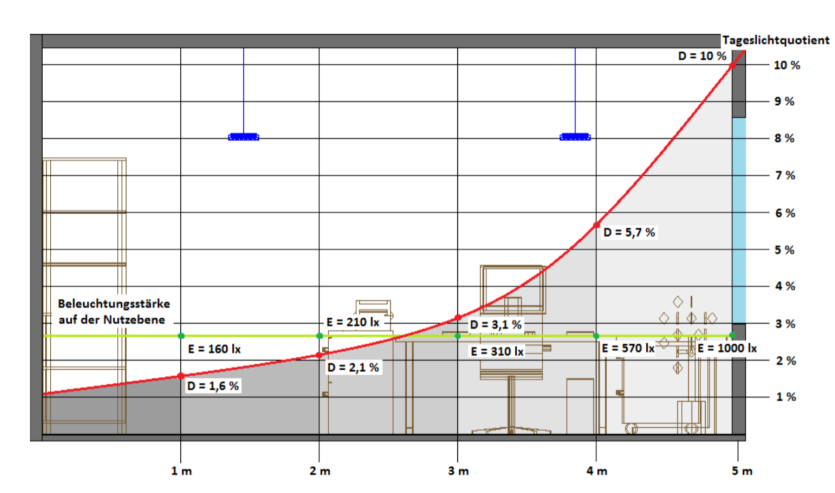
\includegraphics[width=0.7\textwidth]{Abbildungen/abb5.png}
    \caption{Abbildung 5 aus der Versuchsanleitung }
    \label{fig:abb5}
\end{figure}

Die Ergebnisse und die Abbildung unterscheiden sich insofern, dass in den Berechnungen nicht der Tageslichtquotient D, sondern der Transmissionsgrad und die Verminderungs- bzw. Korrekturfaktoren bestimmt wurden.
Dazu kommt, dass die Abbildung die Tiefe des Raumes berücksichtigt während die Berechnungen nur einen einzelnen Wert ergeben. 
Die Berechnungen berücksichtigen dafür durch die zwei unterschiedlichen Szenarien mögliche Schwankungen durch beispielsweise Verschmutzungen der Fenster.

\subsection{Wie würden Sie die Steuerung der Beleuchtung anpassen?}

Prinzipiell reicht die Beleuchtung für die geforderten Bedingungen vollkommen aus.
Man könnte darüber nachdenken nach Sonnenuntergang den Dimmwert der zweiten Steuergruppe auf 25 \% zu senken. Auch eine automatische Dimmung die sich den Lichtbedingungen anpasst könnte erwogen werden.



\subsection{Von welchen baulichen Bedingungen hängt der Himmelslichtanteil DH ab?}

Der Himmelslichtanteil ist von vielen Faktoren abhängig. Dazu zählen:
\begin{itemize}
\item Fenstergröße und Position: größer, weiter oben liegende Fenster lassen mehr Lichteinfall zu als kleinere
\item Umgebung rund um die Fenster bzw. Gebäude: Bäume, Hügel, andere Gebäude usw. können Abschattungen oder Ähnliches verursachen
\item Innenausstattung wie Vorhänge, Rollläden, Farbe der Wände etc. 
\item Wetterbedingungen
\item Transmissionsgrade der Fenster und deren Verschmutzung

\end{itemize}

\subsection{Welche baulichen Maßnahmen könnten ihn verbessern?}
Der Himmelslichtanteil kann durch größere Fenster, den Einbau von Oberlichtern oder Lichtschächten und reflektierende Materialien verbessert werden. Außerdem kann das Fällen von Bäumen vor dem Fenster oder sogar im Extremfall der Abriss eines in der Umgebung befindlichen Gebäudes den Lichteinfall verbessern.

\subsection{Um wie viel reduziert sich Ea, wenn bei gleichmäßig bedecktem Himmel der Horizont
gleichförmig 10° über der Horizontalen liegt?}

Allgemein gesprochen führt eine Erhöhung des Horizonts über der Horizontalen zu einer Verringerung des einfallenden Lichts.
Da bei vollständig bedecktem Himmel davon ausgegangen werden kann, dass der Lichteinfall von überall gleich stark ist muss die wegfallende Fläche durch die Erhöhung des Horizontes berechnet werden. Daraus ergibt sich bei einer Halbkugel von $180^{\circ}-20^{\circ}=160^{\circ}$ was 89 \% des ursprünglichen Wertes entspricht. $E_a$ reduziert sich also um ca. 11 \%. 




